\documentclass[7pt]{article}

\usepackage{fontspec}
\setmainfont[Script=Cyrillic]{Times New Roman}

\usepackage{polyglossia}
\setdefaultlanguage{mongolian}

\usepackage[top=6mm,bottom=6mm,left=6mm,right=6mm]{geometry}
\usepackage{graphicx}
\usepackage{multicol}
\usepackage{amsmath}
\usepackage{float}
\usepackage{indentfirst}
\usepackage{fancyhdr}

% Define necessary commands from Information.tex
\def\titlename{Дижитал тэмдэглэлийн аппликейшн хөгжүүлэх}
\def\departmentname{Компьютерийн ухаал, програм хангамжийн инженерчлэл}
\def\studentID{У2010}
\def\authorShort{Анунаа}
\def\supervisorname{Проф. Дамдины Жаргалсайхан}

\begin{document}

\pagestyle{empty}
\thispagestyle{plain}

\begin{center}
{\large\bfseries \titlename}
\end{center}

{\tiny
\departmentname

Оюутан: \studentID, \authorShort

Удирдагч багш: \supervisorname
}

\setlength{\columnsep}{2mm}

\begin{multicols}{2}

\tiny

\textbf{1. Удиртгал}

Орчин үед хүмүүс өдөр тутмын ажил, хичээл, хувийн төлөвлөгөөгөө тогтмол тэмдэглэх хэрэгцээ өндөр болсон. Гэвч цаасан тэмдэглэл алдагдах эрсдэлтэй, авч явахад хүндрэлтэй байдаг. Иймээс сануулга, календарь болон AI стикер үүсгэх боломжтой ухаалаг дижитал тэмдэглэлийн систем шаардлагатай болсон. Энэхүү ажлаар ``AI Notebook'' системийг боловсруулж хэрэгжүүлэв.

\textbf{Зорилго}

Frontend болон backend-д суурилсан, хэрэглэгчийн баталгаажуулалт, тэмдэглэлийн менежмент, хиймэл оюун ухаанаар стикер үүсгэх боломжтой гар утасны аппликейшн хөгжүүлж ажиллагааг туршилтаар үнэлэх.

\textbf{2. Судалгааны арга зүй}

Энэхүү судалгаанд Design Science Research аргыг ашиглаж шаардлага тодорхойлох, архитектур төлөвлөх, хөгжүүлэлт хийх, турших үе шатуудыг хэрэгжүүлсэн.

\begin{itemize}
\item DFD контекст болон түвшин 1--2
\item Sequence Diagram
\item Интеграцийн тест
\item Гүйцэтгэлийн хэмжилт
\end{itemize}

\textbf{3. Судалгааны үр дүн}

Системийн үндсэн урсгалууд амжилттай баталгаажсан.

\begin{itemize}
\item JWT Authentication
\item CRUD ажиллагаа
\item AI Sticker Generation
\item Push Notification
\end{itemize}

Generative AI туршилтаар fallback, designed болон cached сценаруудын гүйцэтгэлийг хэмжсэн.

\textbf{4. Дүгнэлт}

AI Notebook системийг амжилттай хэрэгжүүлж тэмдэглэл удирдах болон AI стикер үүсгэх боломжуудыг нэгтгэн туршиж баталгаажуулсан.

\end{multicols}

\newpage

\begin{multicols}{2}

\begin{center}
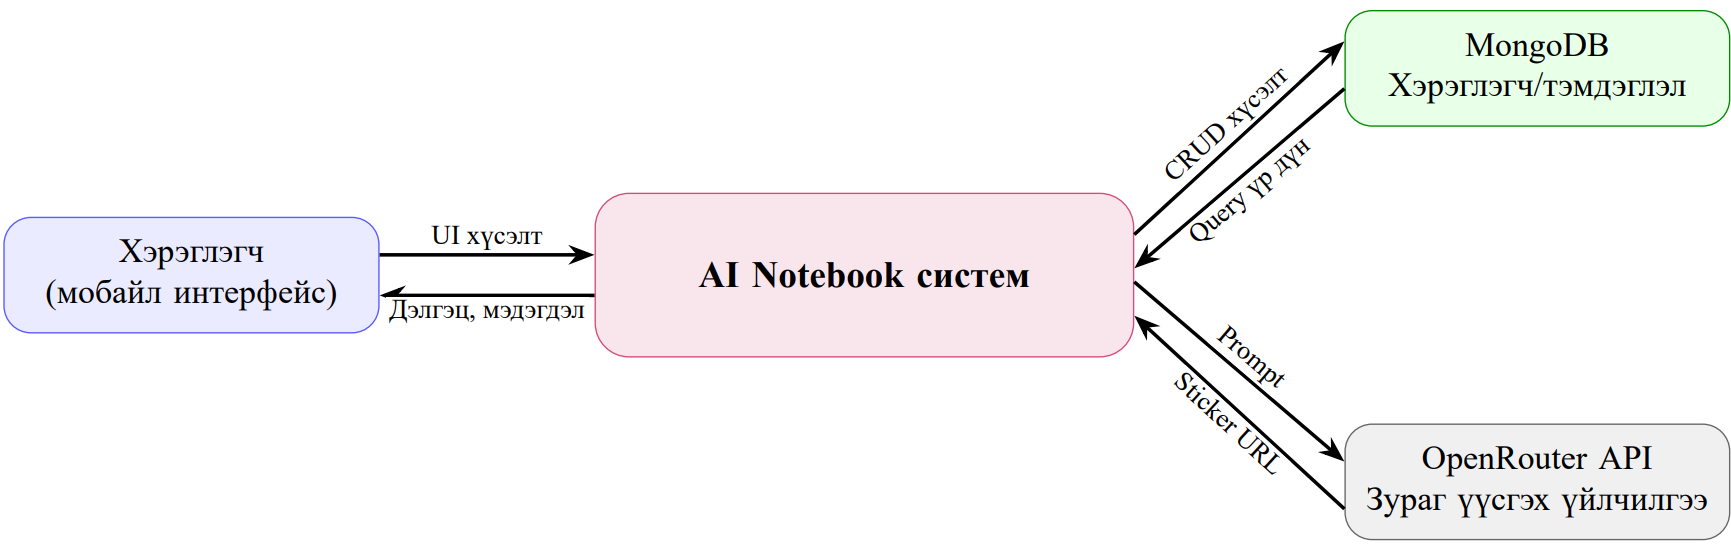
\includegraphics[width=0.95\linewidth]{Pictures/context1.png}

{\scriptsize Зураг 1. Контекст түвшний DFD}
\end{center}

\begin{center}
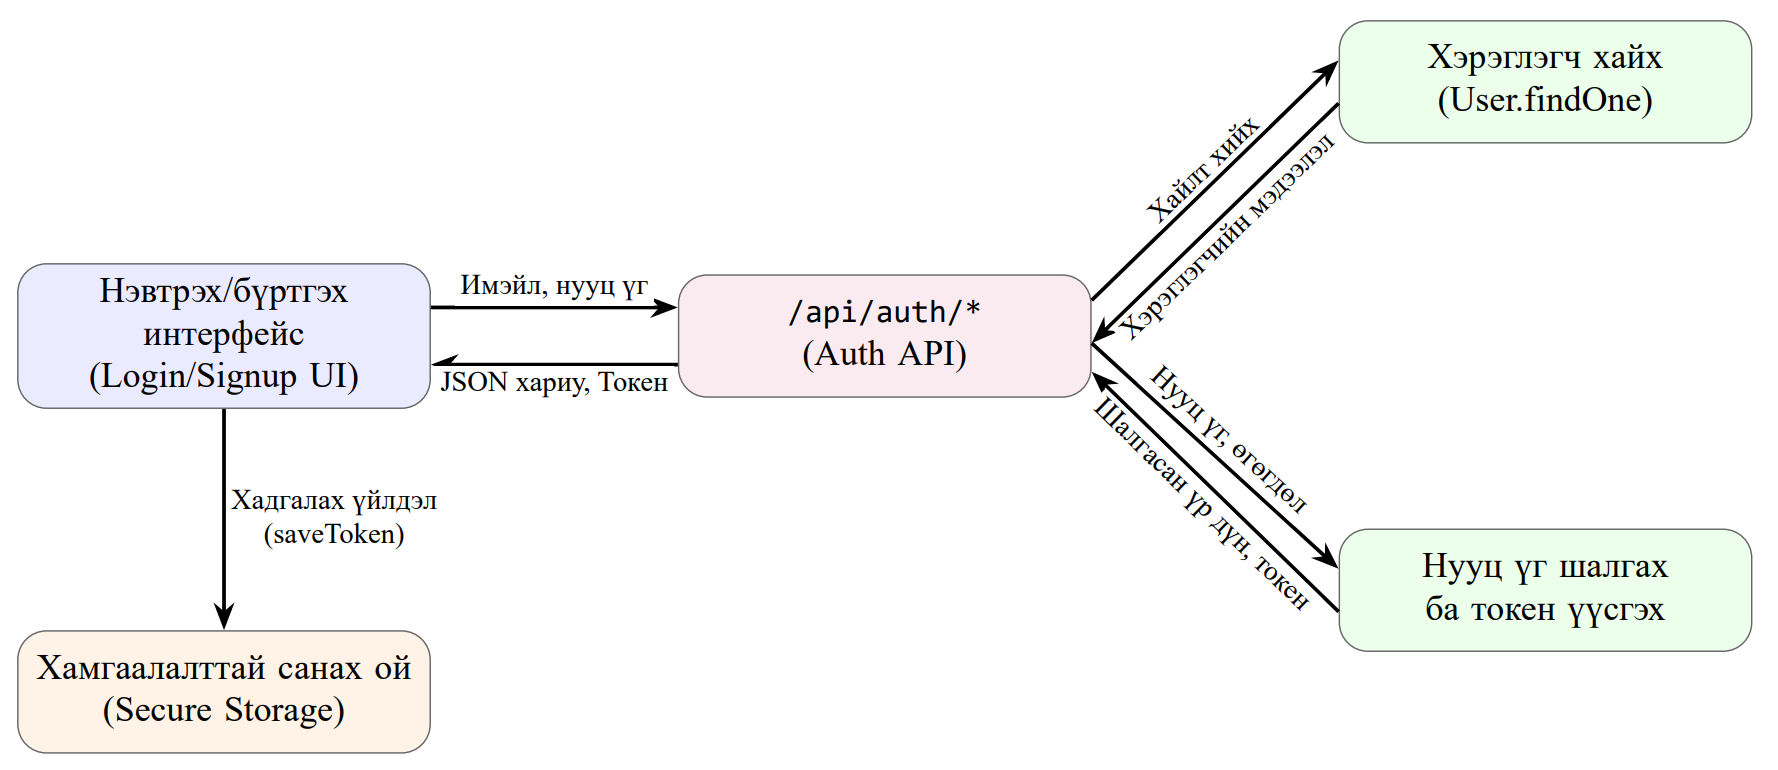
\includegraphics[width=0.95\linewidth]{Pictures/2r_tuvshin2.png}

{\scriptsize Зураг 2. DFD Level 1}
\end{center}

\begin{center}
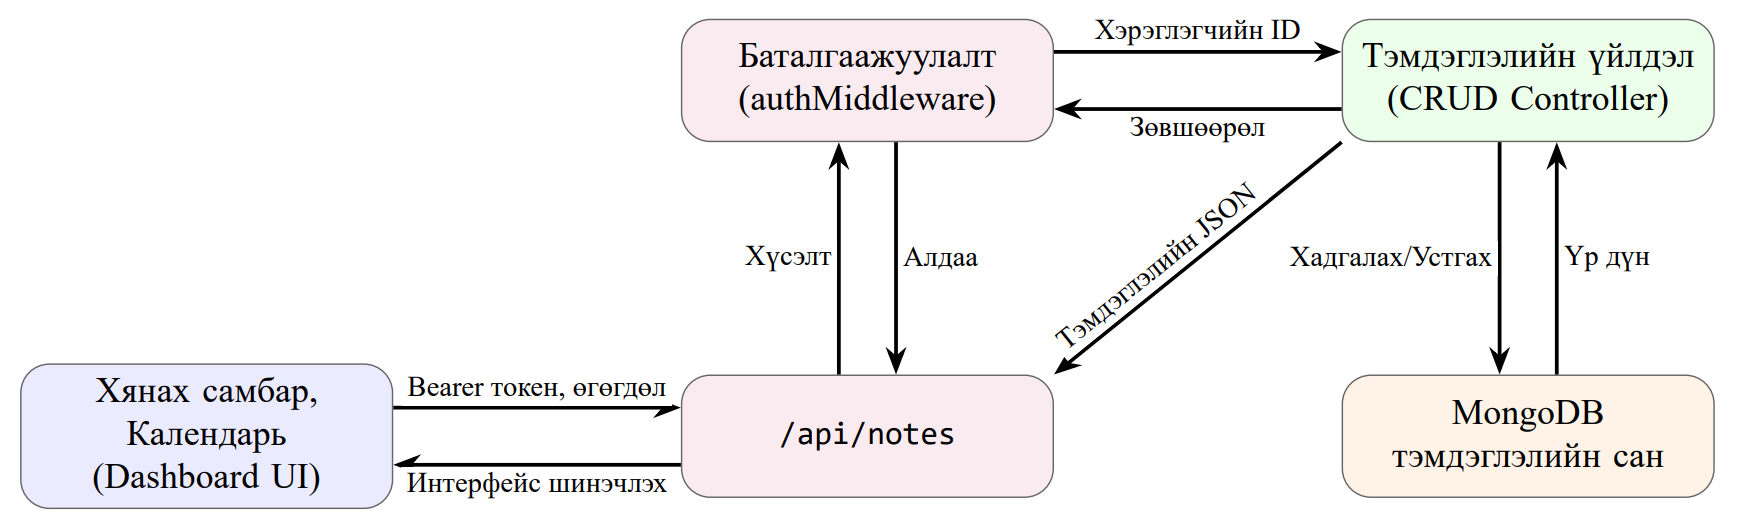
\includegraphics[width=0.95\linewidth]{Pictures/2r_tuvshin_3.png}

{\scriptsize Зураг 3. DFD Level 2}
\end{center}

\columnbreak

\begin{center}
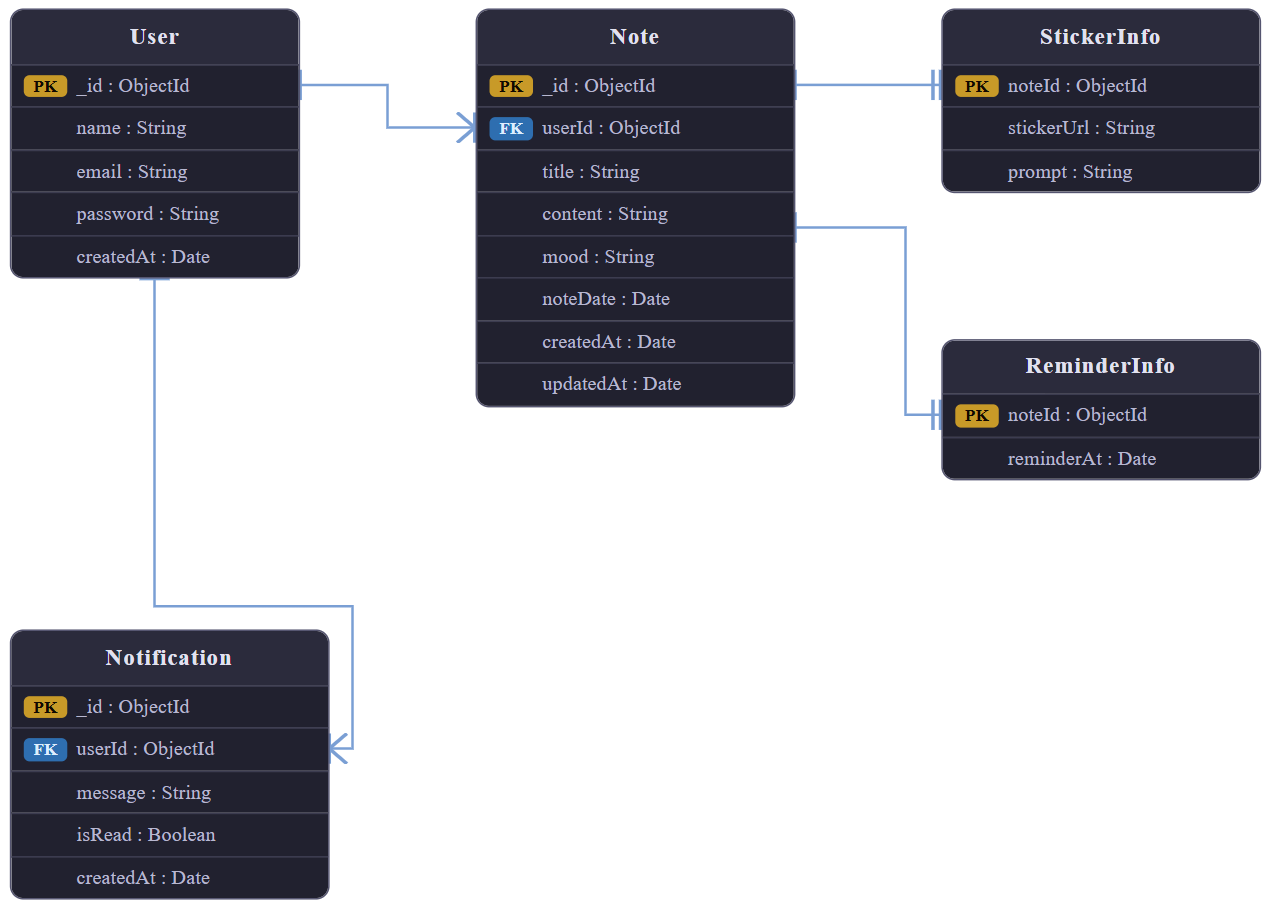
\includegraphics[width=0.95\linewidth]{Pictures/ERD.png}

{\scriptsize Зураг 4. ERD}
\end{center}

\begin{center}
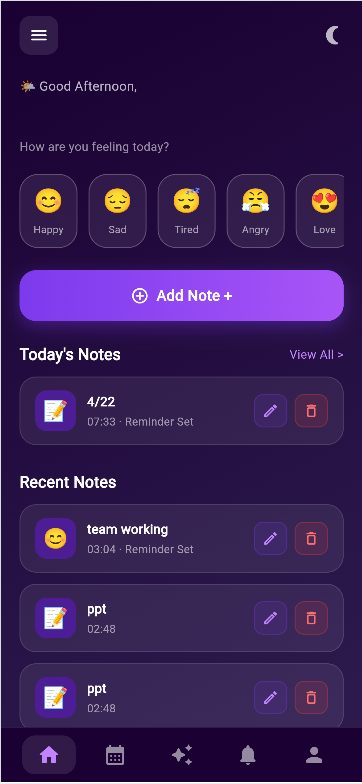
\includegraphics[width=0.95\linewidth]{Pictures/ss_dashboard.png}

{\scriptsize Зураг 5. Dashboard}
\end{center}

\begin{center}
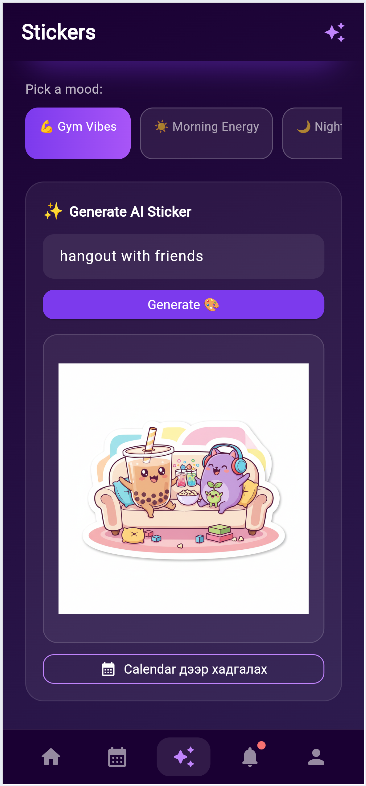
\includegraphics[width=0.95\linewidth]{Pictures/ss_sticker_generation.png}

{\scriptsize Зураг 6. AI Sticker}
\end{center}

\end{multicols}

\end{document}
